\documentclass[10pt,a4paper]{article}
\usepackage[utf8]{inputenc}
\usepackage[top=20mm, left=20mm, bottom=20mm, right=20mm]{geometry}
\usepackage{svg}
\usepackage{graphicx}
\usepackage{caption}
\usepackage{subcaption}
\usepackage[nosumlimits]{amsmath}
\usepackage{multirow}
\usepackage{array}
\usepackage{float}
%\usepackage[table]{xcolor}
\usepackage{longtable}
\usepackage{tabularx}
\usepackage{booktabs}
\usepackage{geometry}

\usepackage[
    backend=biber, 
    natbib=true,
    style=numeric,
    sorting=none
]{biblatex}

\addbibresource{references.bib}

\setlength{\parindent}{0em} 

\title{\vspace{.0cm}Urban Systems and Transportation \\ Final Project \vspace{5.5cm}\\ \textbf{Regional Transfers to Fund Resilient Local Communities}\vspace{3.5 cm}}
\author{Jan-Philip Erdmann, Samuel Luther, Nils Renziehausen, \\Ane Nielsen Solberg, Nicolas Y.C. Triebold\vspace{1cm}}
\date{December 2022}

\begin{document}
\pagenumbering{gobble}
\maketitle
\newpage
\pagenumbering{arabic}

%\section{Table of Contents}

%\newpage
\begin{abstract}
Abstract of report
\end{abstract}
\newpage
\section{Introduction}
As part of the autumn semester 2022 course \textit{Urban Systems and Transportation} at ETH Zurich \cite{course}, we have executed research looking into the effects of climate change related exposures on regions of the United Kingdom (UK), defined and calculated local and external economical costs, and build a model which simulates the reaction of individuals and firms to transfers. The model explores different transfer strategies and are evaluated by the metrics and welfare function. \\\\
Strategies for regional transfers to fund resilient local communities are important to ...
\\\\
In accordance with the given assignment specifications for the final project, we have decided to focus on the UK and build an economical cost model based on risk factors for climate change exposures, as well as transportation and infrastructure assets. The report compares geographical locations at the regional first level NUTS (nomenclature d'unités territoriales statistiques)\cite{2022firstlevel,noauthor_international_2022}, as seen in the map and list of statistical regions in figure \ref{fig:ITLUk}.\\
\begin{figure}[H]\hspace{1.25cm}
  %\centering
  \begin{minipage}{.5\textwidth}\hspace{.75cm}
      %\centering
      \resizebox{0.8\textwidth}{!}{\includesvg[width=200pt]{NUTS_1_statistical_regions_of_the_United_Kingdom_map.svg}}
  \end{minipage}%
  \begin{minipage}{.5\textwidth}
    \vspace{-1cm}
    \begin{itemize}
            \item[] \hspace{-.5cm}\textbf{Legend:}
            \item[]
            \item \textbf{C} North East England
            \item \textbf{D} North West England
            \item \textbf{E} Yorkshire and the Humber
            \item \textbf{F} East Midlands
            \item \textbf{G} West Midlands
            \item \textbf{H} East of England
            \item \textbf{I} London
            \item \textbf{J} South East England
            \item \textbf{K} South West England
            \item \textbf{L} Wales
            \item \textbf{M} Scotland
            \item \textbf{N} Northern Ireland
        \end{itemize}
    \end{minipage}
    \vspace{.25cm}
    \caption{ITL - statistical first level NUTS regions in the UK 
    \label{fig:ITLUk}
    \cite{zotero-176}}
\end{figure}
\newpage
\section{Data Collection} \label{sec:data}

\subsection{Risk Data}
Risk data was gathered in order to define the exposure of climate changes occurring in relation to different sets of assets. An overview of the risk data is represented in table \ref{tab:riskdata}.

\begin{table}[H]
\centering
\begin{tabular}{|l|>{\raggedleft\arraybackslash}m{2cm}|>{\raggedleft\arraybackslash}m{2cm}|>{\raggedleft\arraybackslash}m{1.3cm}|>{\raggedleft\arraybackslash}m{2cm}|>{\raggedleft\arraybackslash}m{1.3cm}|}
\hline
     Region & \multicolumn{1}{|p{2cm}|}{Temperature Increase [$C$]} & \multicolumn{1}{|p{2cm}|}{Rain [$mm$]} & \multicolumn{1}{|p{1.3cm}|}{Flood Risk [\%]} & \multicolumn{1}{|p{2cm}|}{$CO_2$ Emiss- ions [$kt CO_2$]} & \multicolumn{1}{|p{1.3cm}|}{Fire Risk [$-$]} \\
     \hline
     North East England & 1.310216618 & 34.64543189 & 0.16 & 14821.2 & - \\\hline
    North West England & 1.234132058 & 47.9029482 & 0.11 & 41921.9 & - \\\hline
    Yorkshire and the Humber & 1.563126672 & 33.81479328 & 0.69 & 36938.7 & - \\\hline
    East Midlands & 1.05967585 & 28.5870585 & 0.22 & 30197.7 & - \\\hline
    West Midlands & 0.931622388 & 31.71592436 & 0.07 & 31551.8 & - \\\hline
    East of England & 1.586752957 & 26.11977272 & 0.08 & 36562.2 & - \\\hline
    London & 1.703314869 & 29.98249621 & 0.10 & 28369.3 & - \\\hline
    South East England & 1.370755049 & 35.48214576 & 0.14 & 40399.6 & - \\\hline
    South West England & 0.718199346 & 45.66582055 & 0.17 & 30372.1 & - \\\hline
    Wales & 0.710093123 & 58.76975534 & 0.11 & 27303 & - \\\hline
    Scotland & 0.83530936 & 54.7447184 & 0.07 & 37944.7 & - \\\hline
    Northern Ireland & 0.490934677 & 39.6731276 & 0.07 & 21145.7 & - \\
    \hline
\end{tabular}
\caption{Risk Data}
\label{tab:riskdata}
\end{table}
\vspace{-.5cm}
\subsubsection{Temperature Increase}
United Kingdom Climate Projections User Interface (UKCP UI) provides tools and data of the latest updates for climate projections, enabling users to follow future climate trends in the UK. The service provide regional, global, probabilistic, marine and derived projections. Their website offered the possibility to download data observed from weather stations from HadUK-Grid. We downloaded annually mean temperature data and compared the average temperature for the first 10 years of the data set with the average temperature for the last 10 years. The value for the increase is the difference.  
\cite{noauthor_uk_nodate}
\subsubsection{Rainfall}
As UKCP UI provide data on climate projections, we used the same dataset as for temperature for gathering data of the monthly rainfall in $mm$ from 1962-2020 and calculated the standard deviation using the N method for each region of the UK. \cite{noauthor_uk_nodate}
\subsubsection{Flood Risk}
The gov.uk official statistics website offers data on floods and flood risk and it provides the possibility for reviewing the long-term flood risk exposure for each postal code in the UK. The data contains a percentage value for the probability for a flooding event in the next year. The underlying data set has been extracted. An additional data set mapping the millions of postal codes to the NUTS regions was used to derive the average flood risk in each region. The Jupyter Notebook can be found in the additional materials in the folder containing the raw data for the flood risk. \cite{noauthor_open_nodate,noauthor_postcode_nodate}
\subsubsection{$CO_2$ Emissions}
Regional $CO_2$ emissions data from 2005 to 2019 could be directly sourced and downloaded from the official gov.uk statistics website. \cite{uk,ukc}
\subsubsection{Fire Risk}
Regional fire risk data was difficult to detect. The only usable data we could access was charts denoting the fire number and burnt area per year for England, North Ireland, Scotland and Wales. These were manually transcribed, but not further used. \cite{countryprofile}

\subsection{Asset Data}
Asset data were gathered to define a set of available resources with economical value in the UK regions as well as population data. The value of the resources available and risks related to climate change on the specific asset will define what costs an exposure will inflict. An overview of the asset values is represented in tables \ref{assetdata1} and \ref{assetdata2}.

% \begin{table}[H]
% \centering
% \label{asset data}
% \begin{tabular}{|l|>{\raggedleft\arraybackslash}m{1.6cm}|>{\raggedleft\arraybackslash}m{1.6cm}|>{\raggedleft\arraybackslash}m{1.6cm}|>{\raggedleft\arraybackslash}m{1.8cm}|>{\raggedleft\arraybackslash}m{1.8cm}|>{\raggedleft\arraybackslash}m{1.7cm}|>{\raggedleft\arraybackslash}m{1.7cm}|>{\raggedleft\arraybackslash}m{2.5cm}|>{\raggedleft\arraybackslash}m{2.5cm}|>{\raggedleft\arraybackslash}m{2.5cm}|}
% \hline
% Region & \multicolumn{1}{|p{1.6cm}|}{GDP [$Mil$$GBP$]}& \multicolumn{1}{|p{1.6cm}|}{Motorways [$Miles$]} & \multicolumn{1}{|p{1.6cm}|}{Road/Rail [$Travel Time$]}& \multicolumn{1}{|p{1.8cm}|}{Ports [$MT/year$]}& \multicolumn{1}{|p{1.8cm}|}{Energy Generation [$GWh$]}& \multicolumn{1}{|p{1.7cm}|}{Agriculture [$Hectars$]} & \multicolumn{1}{|p{1.7cm}|}{Population [\#]}& Area [$km^2$] & Population density [$population/km$] & Wage [$GBP$] \\\hline
% North East England & 61951 & 36 & 61657549 & 58.694167 & 11225.23452 & 641820 & 2680763 & 8592 & 312.0068669 & 575.2 \\\hline
% North West England & 208183 & 408 & 7367456	155.04227 & 30849.95213 & 1066920 & 7367455 & 14165 & 520.1168373 & 602.3 \\\hline
% Yorkshire and the Humber & 142008 & 277 & 143685100 & 174.13554 & 23140.64123 & 1204530 & 5526350 & 15420 & 358.3884565 & 579.1 \\\hline
% East Midlands & 126289 & 124 & 111908409 & 1.606792 & 20373.79294 & 1204620 & 4865583 & 15627 & 311.3574582	594.1 \\\hline
% West Midlands & 156685 & 277 & 155010154 & 0 & 24964.55347 & 942730 & 5961929 & 12998 & 458.6804893 & 617.5 \\\hline
% East of England & 182910 & 165 & 156729025 & 164.128696 & 26251.03469 & 1412160 & 6269161 & 19120 & 327.8849895 & 632.4 \\\hline
% London & 503904 & 37 & 414114448 & 156.406244 & 37696.37193 & 12690 & 9002488 & 1569 & 5737.723391 & 804.9 \\\hline
% South East England & 318142 & 410 & 239648890 & 798.040509 & 38595.71372 & 1174100 & 9217265 & 19095 & 482.7056821 & 664.3 \\\hline
% South West England & 158524 & 204 & 130160289 & 49.429954 & 23696.68911 & 1853350 & 5659143 & 3800 & 237.7791176	611.3 \\\hline
% Wales & 75695 & 88 & 69730892 & 184.635805 & 28608.34494 & 1741260 & 3169586 & 20779 & 152.537947 & 598.1 \\\hline
% Scotland & 161954 & 295 & 142116000 & 181.810821 & 49969.43158 & 5984840 & 5466000 & 77933 & 70.13716911 & 640.5 \\\hline
% Northern Ireland & 48478 & 70 & 53074280 & 177.186172 & 9389.178643 & 1055430 & 1895510 & 14130 & 134.1479122 & 591.6 \\\hline
% \end{tabular}
% \caption{Asset Data}
% \end{table}

\begin{table}[H]
\centering
\begin{tabular}{|l|>{\raggedleft\arraybackslash}m{1.8cm}|>{\raggedleft\arraybackslash}m{1.6cm}|>{\raggedleft\arraybackslash}m{2.4cm}|>{\raggedleft\arraybackslash}m{2cm}|>{\raggedleft\arraybackslash}m{2.2cm}|}
\hline
Region & \multicolumn{1}{|p{1.8cm}|}{GDP \quad[$Mil$ $GBP$]}& \multicolumn{1}{|p{1.6cm}|}{Motorways [$Miles$]} & \multicolumn{1}{|p{2.4cm}|}{Road/Rail [$Travel$ $Time$]}& \multicolumn{1}{|p{2.cm}|}{Ports [$MT/year$]}& \multicolumn{1}{|p{2.2cm}|}{Energy Gene- ration [$GWh$]}\\\hline
North East England & 61'951 & 36 & 61'657'549 & 58.694167 & 11'225.23452 \\\hline
North West England & 208'183 & 408 & 7'367'456	& 155.04227 & 30'849.95213 \\\hline
Yorkshire and the Humber & 142'008 & 277 & 143'685'100 & 174.13554 & 23'140.64123\\\hline
East Midlands & 126'289 & 124 & 111'908'409 & 1.606792 & 20'373.79294\\\hline
West Midlands & 156'685 & 277 & 155'010'154 & 0 & 24'964.55347 \\\hline
East of England & 182'910 & 165 & 156'729'025 & 164.128696 & 26'251.03469 \\\hline
London & 503'904 & 37 & 414'114'448 & 156.406244 & 37'696.37193 \\\hline
South East England & 318'142 & 410 & 239'648'890 & 798.040509 & 38'595.71372\\\hline
South West England & 158'524 & 204 & 130'160'289 & 49.429954 & 23'696.68911 \\\hline
Wales & 75'695 & 88 & 69'730'892 & 184.635805 & 28'608.34494 \\\hline
Scotland & 161'954 & 295 & 142'116'000 & 181.810821 & 49'969.43158 \\\hline
Northern Ireland & 48'478 & 70 & 53'074'280 & 177.186172 & 9389.178643 \\\hline
\end{tabular}
\caption{Asset Data, Part 1}
\label{assetdata1}
\end{table}
\vspace{-.5cm}
\begin{table}[H]
\centering
\begin{tabular}{|l|>{\raggedleft\arraybackslash}m{1.9cm}|>{\raggedleft\arraybackslash}m{1.8cm}|>{\raggedleft\arraybackslash}m{1.1cm}|>{\raggedleft\arraybackslash}m{3.2cm}|>{\raggedleft\arraybackslash}m{2cm}|}
\hline
Region & \multicolumn{1}{|p{1.9cm}|}{Agriculture [$Hectars$]} & \multicolumn{1}{|p{1.8cm}|}{Population [\#]}& \multicolumn{1}{|p{1.1cm}|}{Area [$km^2$]} & \multicolumn{1}{|p{3.2cm}|}{Population Density [$population/km^2$]} & \multicolumn{1}{|p{2cm}|}{Wage [$GBP/week$]} \\\hline
North East England & 641'820 & 2'680'763 & 8592 & 312.0068669 & 575.2 \\\hline
North West England & 1'066'920 & 7'367'455 & 14'165 & 520.1168373 & 602.3 \\\hline
Yorkshire and the Humber & 1'204'530 & 5'526'350 & 15'420 & 358.3884565 & 579.1 \\\hline
East Midlands & 1'204'620 & 4'865'583 & 15'627 & 311.3574582	& 594.1 \\\hline
West Midlands & 942'730 & 5'961'929 & 12'998 & 458.6804893 & 617.5 \\\hline
East of England & 1'412'160 & 6'269'161 & 19'120 & 327.8849895 & 632.4 \\\hline
London & 12'690 & 9'002'488 & 1569 & 5737.723391 & 804.9 \\\hline
South East England & 1'174'100 & 9'217'265 & 19'095 & 482.7056821 & 664.3 \\\hline
South West England & 1'853'350 & 5'659'143 & 3800 & 237.7791176	& 611.3 \\\hline
Wales & 1'741'260 & 3'169'586 & 20'779 & 152.537947 & 598.1 \\\hline
Scotland & 5'984'840 & 5'466'000 & 77'933 & 70.13716911 & 640.5 \\\hline
Northern Ireland & 1'055'430 & 1'895'510 & 14'130 & 134.1479122 & 591.6 \\\hline
\end{tabular}
\caption{Asset Data, Part 2}
\label{assetdata2}
\end{table}
\vspace{-.5cm}
\subsubsection{GDP}
GDP was used as a measure of the size of the regional economies. ons.gov.uk provide estimates of regional GDP for all ITL regions data sets available for download. \cite{regional}
\subsubsection{Motorway Infrastructure}
gov.uk publish data and statistics on road conditions, including motorway data. We collected data about miles of motorway in the UK regions. Northern Ireland was lacking in the gov.uk dataset and was collected by multiplying the miles of each motorway from Wikipedia.
\cite{road,noauthor_categorymotorways_2013}%,2022roads}
\subsubsection{Port Infrastructure}
gov.uk publish port and domestic waterborne freight statistics produced by Department of Transport. We gathered the data for all freight (million) gross tonnage traffic by port and year and divided them by the region of placement.
\cite{port}
\subsubsection{Energy Generation}
The electricity generated in each region was collected from gov.uk publication for energy trends. In the dataset we accessed there was a total value for England and not divided into regions. Therefore, we distributed the total GWh energy generation on the regions based on population, assuming that the amount of energy generated for a region is in correlation with the population. 
\cite{energy}
\subsubsection{Agricultural Land use}
Land used for agriculture were gathered form eurostat Data Browser for Farm structure and Farm land use for NUTS 2 regions in the UK. The values for hectars Farm land were added together for the NUTS 1 regions.
\cite{statistics}
\subsubsection{Population}
The population for each region were selected from Statista in absolute numbers. The population density was derived by dividing the absolute numbers by the area of the region. \cite{noauthor_uk_nodate,regional,uk,noauthor_international_2022}
\subsubsection{Area}
The area was collected as $km^2$ from the Wikipedia page for International Territorial Level NUTS 1 regions of UK.
\cite{noauthor_international_2022,regional,uk}
\subsubsection{Income}
The median weekly income for full-time employees in UK by regions was collected from Statista.
\cite{fulltime,2022list}

\section{Monetary Value and Risk Estimation}
\subsection{Valuation of Assets}
%\cite{ukb,uka,total,2022list}
The value estimations is represented in table \ref{assetvalue}.

\begin{table}[H]
    \centering
    \begin{tabular}{|l|>{\raggedleft\arraybackslash}m{2.3cm}|>{\raggedleft\arraybackslash}m{2.2cm}|>{\raggedleft\arraybackslash}m{2.5cm}|>{\raggedleft\arraybackslash}m{2.7cm}|}
    \hline
    %\multicolumn{5}{|c|}{}\\
    %\multicolumn{5}{|c|}{Value of assets in $GBP$}\\
    %\multicolumn{5}{|c|}{}\\\hline
    Region & \multicolumn{1}{|p{2.3cm}|}{Ports} & \multicolumn{1}{|p{2.2cm}|}{Motorway \quad Infrastructure} & \multicolumn{1}{|p{2.5cm}|}{Agricultural Land} & \multicolumn{1}{|p{2.7cm}|}{Energy\quad\quad\quad Generation}\\\hline
North East England & 17'494'388'777 & 1'080'000'000 & 393'698'856.21 &  2'254'622'029.91 \\\hline
North West England & 46'211'913'158 & 12'240'000'000 & 654'459'480.33  &  6'196'305'435.18 \\\hline
Yorkshire and the Humber & 51'902'854'958 & 8'310'000'000 & 738'870'841.16 & 4'647'867'213.54 \\\hline
East Midlands & 478'920'570	& 3'720'000'000 & 738'926'048.06 & 4'092'137'432.56 \\\hline
West Midlands & 0 & 8'310'000'000 & 578'280'082.76 & 5'014'205'457.23 \\\hline
East of England & 48'920'214'122 & 4'950'000'000 & 866'233'175.64 & 5'272'599'069.60 \\\hline
London & 46'618'459'373 & 1'110'000'000 & 7'784'173.89 & 7'571'429'391.10 \\\hline
South East England & 237'864'027'008 & 12'300'000'000 & 720'204'772.49 & 7'752'064'887.67 \\\hline
South West England & 14'733'096'604 & 6'120'000'000 & 1'136'863'567.91 & 4'759'551'097.28 \\\hline
Wales & 55'032'564'903 & 2'640'000'000 & 1'068'106'432.28 & 5'746'071'907.04\\\hline
Scotland & 54'190'549'914 & 8'850'000'000 & 3'671'161'170.74 & 10'036'510'241.68 \\\hline
Northern Ireland & 52'812'126'611 & 2'100'000'000 & 647'411'398.54 & 1'885'844'698.04    \\\hline   
    \end{tabular}
    \caption{Valuation of assets in $GBP$}
    \label{assetvalue}
\end{table}

% \begin{table}[H]
%     \centering
%     \begin{tabular}{|l|>{\raggedleft\arraybackslash}m{2.3cm}|>{\raggedleft\arraybackslash}m{2.2cm}|>{\raggedleft\arraybackslash}m{2.4cm}|>{\raggedleft\arraybackslash}m{2.5cm}|>{\raggedleft\arraybackslash}m{2.2cm}|>{\raggedleft\arraybackslash}m{2.2cm}|}
%     \hline
%     \multicolumn{7}{|c|}{}\\
%     \multicolumn{7}{|c|}{Value of assets / risks in $pounds$}\\
%     \multicolumn{7}{|c|}{}\\\hline
%     Region & \multicolumn{1}{|p{2.3cm}|}{Ports} & \multicolumn{1}{|p{2.2cm}|}{Motorway Infrastructure} & \multicolumn{1}{|p{2.4cm}|}{Agricultural Land} & \multicolumn{1}{|p{2.5cm}|}{Energy Generation}& \multicolumn{1}{|p{2.2cm}|}{Private Wealth} & $CO_2$\\\hline
% North East England & 17'494'388'777 & 1'080'000'000 & 393'698'856.21 &  2'254'622'029.91 & 3.1403E+11 & 1'067'126'400 \\\hline
% North West England & 46'211'913'158 & 12'240'000'000 & 654'459'480.33  &  6'196'305'435.18 & 1.05528E+12 & 3'018'376'800 \\\hline
% Yorkshire and the Humber & 51'902'854'958 & 8'310'000'000 & 738'870'841.16 & 4'647'867'213.54 & 7.19839E+11 & 2'659'586'400 \\\hline
% East Midlands & 478'920'570	& 3'720'000'000 & 738'926'048.06 & 4'092'137'432.56 & 6.40159E+11 & 2174234400 \\\hline
% West Midlands & 0 & 8'310'000'000 & 578'280'082.76 & 5'014'205'457.23 & 7.94236E+11 & 2271729600 \\\hline
% East of England & 48'920'214'122 & 4'950'000'000 & 866'233'175.64 & 5'272'599'069.60 & 9.27171E+11 & 2'632'478'400 \\\hline
% London & 46'618'459'373 & 1'110'000'000 & 7'784'173.89 & 7'571'429'391.10 & 2.55429E+12 & 2'042'589'600 \\\hline
% South East England & 237'864'027'008 & 12'300'000'000 & 720'204'772.49 & 7'752'064'887.67 & 1.61266E+12 & 2'908'771'200 \\\hline
% South West England & 14'733'096'604 & 6'120'000'000 & 1'136'863'567.91 & 4'759'551'097.28 & 8.03558E+11 & 2'186'791'200 \\\hline
% Wales & 55'032'564'903 & 2'640'000'000 & 1'068'106'432.28 & 5'746'071'907.04 & 3.83698E+11 & 1'965'816'000 \\\hline
% Scotland & 54'190'549'914 & 8'850'000'000 & 3'671'161'170.74 & 10'036'510'241.68 & 8.20945E+11 & 2'732'018'400 \\\hline
% Northern Ireland & 52'812'126'611 & 2'100'000'000 & 647'411'398.54 & 1'885'844'698.04 & 2.45735E+11 & 1'522'490'400    \\\hline   
%     \end{tabular}
%     \caption{Valuation of assets}
%     \label{assetvalue}
% \end{table}
\vspace{-.5cm}
\begin{itemize}
    %\item The assumption is that the productivity is an inherent property of the regions and does not change with the population density. The productivity was derived by dividing the GDP in each region by the population in the region. \textcolor{red}{control, not needed in the table!}
    \item Value of ports: gov.uk post data about the the total value of goods traded through UK ports in 2014. The value was 29.2 per cent of the GDP in 2014 and for simplicity there was made an assumption that this ratio is constant. Hence, the total value of all ports in our data set was assumed to be 29.2 per cent of the total GDP. We calculated the share of tonnage for each region and then multiplied by 29.2 per cent of total GDP. \cite{uka}
    \item Value of motorway infrastructure: We found the average cost per mile of new motorways in the UK from a BBC article. This value of 30 million pounds was multiplied by each regions value for miles of motorway. This gave an estimation of the value of motorways in each region of the UK. \cite{noauthor_uks_2011}
    \item Value of agricultural land: gov.uk post data about total income from farming in the UK, where we found that in total agriculture's' contribution to the UK economy was £11'222 million in 2021. We used this total value for calculating the mean value of 1 $km^2$ agriculture land, and then we multiplied with each region square meters to get an value estimation for agriculture land in each region. \cite{total}
    \item Energy generation: Statista provide electricity prices from 2010 to 2020. We used the average energy price for 2020 in GBP per GWh and multiplied with the total energy production in GWh for each region, resulting in an estimation of the total energy value for each region. \cite{ukb}
    
    %%\item Private wealth: The wealth-to-GDP ratio as a measure of capital efficiency was collected from Wikipedia for the UK. To estimate a value of the total wealth in each region the ratio was multiplied with the million pound GDP value of each region. We are aware that GDP is not an optimal measure of wealth, but it gives a good estimation for economical transactions in this model.
\end{itemize}

\subsection{Risk Estimation and Valuation}

    To quantify and therefore compare the different risk categories, we connected the different categories to the identified assets and calculated the resulting risk valuation. The calculation steps are explained in the following.
    First, every team member independently estimated the effect of each identified risk on the given assets which are explained in \ref{sec:data} (??). The identified risks are the following:
    \begin{itemize}  
        \item Temperature increase risk
        \item Rain risk
        \item Flood risk
        \item Emissions risk (CO2 cost \cite{noauthor_uk_2022}) (do we need source here?)
    \end{itemize}
    The scale used for the influence estimation reaches from 0 - no influence to 3 - very high influence. The calculated influence is then the average of the different estimations. To check the validity of the estimations, each standard deviation is calculated. The influence values were then scaled to an overall scale of 0 to 1, meaning that the highest value of the whole table is 1 while the lowest for the whole table is 0. The calculated influences can be seen in table \ref{est mean}.
    \begin{table}[H]
    \centering
    \begin{tabular}{|l|l|l|l|l|}
    \hline
                         & Road/Rail Infrastructure & Ports & Energy Generation & Land use of Agriculture \\ \hline
    Temperature increase & 0.2                      & 0.33  & 0.53              & 1                       \\ \hline
    Rain                 & 0.67                     & 0.4   & 0.47              & 1                       \\ \hline
    Flood risk           & 0.87                     & 0.93  & 0.67              & 0.87                    \\ \hline
    CO2 emissions        & 0.13                     & 0.13  & 0.4               & 0.4                    
    \\ \hline
    \end{tabular}
    \caption{Mean values of influence estimations}
    \label{est mean}
    \end{table}
    \vspace{-.0cm}
    The standard deviations are based on the original estimation scale of 0 to 4 and can be seen in Table \ref{est dev}.
    \begin{table}[H]
    \centering
    \begin{tabular}{|l|l|l|l|l|}
    \hline
                         & Road/Rail Infrastructure & Ports & Energy Generation & Land use of Agriculture \\ \hline
    Temperature Increase & 0.8                      & 0.63  & 0.49              & 0                       \\ \hline
    Rain                 & 0.63                     & 0.4   & 0.8               & 0                       \\ \hline
    Flood risk           & 0.49                     & 0.4   & 0                 & 0.88                    \\ \hline
    CO2 emissions        & 0.49                     & 0.49  & 1.17              & 0.75                 
    \\ \hline
    \end{tabular}
    \caption{Standard deviation of influence estimations}
    \label{est dev}
    \end{table}
    \vspace{-.0cm}
    
    Analyzing these values, it is visible that the standard deviation for $CO_2$ emissions influence on energy generation is high (above 1), referring to more spread data values. This could be a result of a different understanding of the influence of emissions in relation to energy generation, and further this makes the data less reliable. The interpretation can either be that the emission is necessary to produce energy or that it has a negative effect on energy generation. All values, also the questionable ones, are considered in the subsequent steps of the calculation.\\
    To achieve an equal non-monetary valuation without units of each risk as a basis for the monetary evaluation, we scaled each risk category to a value between 0 and 1. This value is seen as the relative probability of occurrence. Table \ref{scaled risk} shows the scaled values for each region.

    \begin{table}[H]
    \centering
    \begin{tabular}{|l|l|l|l|l|}
    \hline
    Region                   & Temperature   Increase & Rain        & Flood Risk  & CO2 Emissions \\ \hline
    North East England       & 0.769215746            & 0.589511249 & 0.231884058 & 0.353543136   \\ \hline
    North West England       & 0.724547223            & 0.815095246 & 0.15942029  & 1             \\ \hline
    Yorkshire and the Humber & 0.91769684             & 0.575377472 & 1           & 0.881131342   \\ \hline
    East Midlands            & 0.622125638            & 0.486424664 & 0.31884058  & 0.720332332   \\ \hline
    West Midlands            & 0.546946666            & 0.539664053 & 0.101449275 & 0.752632872   \\ \hline
    East of England          & 0.931567607            & 0.444442427 & 0.115942029 & 0.872150356   \\ \hline
    London                   & 1                      & 0.510168811 & 0.144927536 & 0.676717897   \\ \hline
    South East England       & 0.804757285            & 0.6037484   & 0.202898551 & 0.963687237   \\ \hline
    South West England       & 0.421648022            & 0.777029278 & 0.246376812 & 0.724492449   \\ \hline
    Wales                    & 0.416888936            & 1           & 0.15942029  & 0.651282504   \\ \hline
    Scotland                 & 0.490402201            & 0.931511763 & 0.101449275 & 0.905128346   \\ \hline
    Northern Ireland         & 0.288223091            & 0.675060282 & 0.101449275 & 0.504407004   \\ \hline
    \end{tabular}
    \caption{Scaled risk data}
    \label{scaled risk}
    \end{table}
    
    The next step was to aggregate the asset valuations using the multipliers to calculate a monetary estimation for risk. The risk value \textit{rv} is computed using Equation \ref{risk valuation} with assets \textit{a} and risks \textit{r} for regions \textit{i} using the given parameters risk probability \textit{rp}, asset valuation \textit{av} and influence factor \textit{if}.
    \begin{equation}
        rv_{r,i} = rp_{r,i}*\sum_{a}{if_{r,a}*av_{a,i}}
        \label{risk valuation}
    \end{equation}
    This results to a valuation of each risk in the given regions. For the further model, we aggregated the monetary valuations to simplify the complexity of the whole model using Equation \ref{risk aggregation}.
    \begin{equation}
        rv_{i} = \sum_{r}{rv_{r,i}}
        \label{risk aggregation}
    \end{equation}
\section{Model}

The model uses the following structure to estimate the welfare after transfer payments and reallocation of people. Index $i$ denotes the ITL region.
The model runs multiple times (t = 10). Each run represents one year. The reason is, a change in population though reallocation of people due to a change in attractiveness with the transfer payments the properties of the region are changing. A changing population has an affect on risk per capita formula \ref{risk per capita} and population density formula \ref{population density} with consequences to all following equations. At each consecutive run the newly crated population allocation in the UK is used to calculate the resulting welfare of the transfer schedule.
\newline
\begin{center}
\textbf{\textit{For t }}$\in$ \textbf{[0,10]:}\vspace{.5cm}


The risk per capita is calculated by formula \ref{risk per capita}. The total estimated risk in formula \ref{risk aggregation} is divided by the population in the respective region:
\begin{equation}
    rpc_{i,t} = \frac{rv_{i}}{population_{i,t-1}}
    \label{risk per capita}
\end{equation}

\begin{center}
    $\downarrow$
\end{center}
The population density is provided by formula \ref{population density}, regional population over regional area:
\begin{equation}
    pd_{i,t} = \frac{population_{i,t-1}}{area_i}
    \label{population density}
\end{equation}

\begin{center}
    $\downarrow$
\end{center}
The following correlation formula \ref{wage pop density} of wages $w_{i,t}$ and population density $pd_{i,t}$ is used to estimate the wage $w_{i,t}$ in each region per year (see figure \ref{dg:wage-pop}):
\begin{equation}
    w_{i,t} = (0.0359*pd_{i,t}+598.74) * 52
    \label{wage pop density}
\end{equation}

\begin{center}
    $\downarrow$
\end{center}
Following correlation formula \ref{housing price} of real estate prices $h_i$ to population density $pd_{i,t}$, wages $w_{i,t}$, and financing rate of over 20 years is found to estimate the yearly amount spend by residents on housing $h_{i,t}$ in each region (see figure \ref{dg:housing-pop}):
\begin{equation}
%unkown at the moment NILS has to tell me
    h_{i,t} = \frac{(0.0014*pd_{i,t}+7.0373) * w_{i,t}}{20}
    \label{housing price}
\end{equation}

\begin{center}
    $\downarrow$
\end{center}
A transfer payment scheme is used to reallocate money from one region to another according to an underlying principle. All transfer schedules have in common that a tax between 0\% and 100\% is applied to the income. Every rate is tired out. Take, for instance, transfer schedule 1 as in formula \ref{transfer schedule 1}: The transferred amount depends only on the regional per capita risk level. See further down for other transfer schedules:
\newline
\newline
\textbf{\textit{For tax }}$\in$ \textbf{[0,100]\%:}\vspace{.5cm}
\begin{equation}
    t_{i,t,tax} = tax * \sum_i w_{i,t} * \frac{rpc_{i,t}}{\sum_i rpc_{i,t}} - tax * w_{i,t}
    \label{transfer schedule 1}
\end{equation}

\begin{center}
    $\downarrow$
\end{center}
The attractiveness of a given regions is provided by formula \ref{attractiveness region}. Factor $b_i$, wage, transfer payment, housing expense, and risk per capita in the region is taken into account: 
\begin{equation}
    v_{i,t,tax} = \frac{b_i*(w_{i,t}+t_{i,t,tax}-h_{i,t})}{rpc_{i,t}}
    \label{attractiveness region}
\end{equation}

\begin{center}
    $\downarrow$
\end{center}
Formula \ref{attractiveness region comparison} gives a comparison of the attractiveness of regions and makes them thereby comparable:
\begin{equation}
    \Pi_{i,t,tax} = \frac{v_{i,t,tax}}{\sum_i v_{i,t,tax}}
    \label{attractiveness region comparison}
\end{equation}

\begin{center}
    $\downarrow$
\end{center}
The attractiveness of a region $\Pi_{i,t,tax}$ leads to a population allocation accordingly with formula \ref{population share}. $H_{total}$ corresponds to the total population of the UK:
\begin{equation}
    H_{i,t,tax} = \Pi_{i,t,tax} * H_{total}
    \label{population share}
\end{equation}

\begin{center}
    $\downarrow$
\end{center}
The productivity of the region is given by formula \ref{productivity} by scaling the population with regional productive factor $pf_i$, where $pf_i = GDP_i / population_{i,t=0}$:
\begin{equation}
%pf_productivity facotr
    A_{i,t,tax} = H_{i,t,tax} * pf_i
    \label{productivity}
\end{equation}

\begin{center}
    $\downarrow$
\end{center}
Total welfare $W$ is the sum of all regional productivities given by formula \ref{total welfare}:
\begin{equation}
    W_{t,tax} = \sum_i A_{i,t,tax}
    \label{total welfare}
\end{equation}
\vspace{.25cm}
%\textbf{\textit{Next tax}}
\newline
\textbf{\textit{Next tax}}
\\
\textbf{\textit{Next t}}
\end{center}

\subsection{Determination of Parameter $b_i$}
To implement the model and make it run following steps were required.
First, the unknown factor $b_i$ in formula \ref{attractiveness region} has to be estimated. We have the assumption that currently the risk is considered by people living in each region, therefore the population given by the model through formula \ref{population share} has to be equal to the actual observed regional population in the UK. Using the formulas \ref{risk per capita} to \ref{population share} in MS-Excel with a Solver with the aim to fulfill formula \ref{solver equation} under variation of $b_i$ the $b_i$ for each region is estimated.
\begin{equation}
    H_i(b_i) \stackrel{!}{=}  H_{actual,i}
    \label{solver equation}
\end{equation}

\subsection{Transfer Schedule 1}
The first transfer schedule is already mentioned previously. See formula \ref{transfer schedule 1} or below.
\begin{equation}
    t_{i,t,tax} = tax * \sum_i w_{i,t} * \frac{rpc_{i,t}}{\sum_i rpc_{i,t}} - tax * w_{i,t}
    \label{transfer schedule 1 again}
\end{equation}
The motivation for this transfer schedule is the idea that we just look at the exposed risk for each region and allocate resources accordingly. Collected funds amount to $tax * \sum_i w_{i,t}$, where every individual contributes with $tax * w_{i,t}$. The redistribution follows the ratio of regional per capita risk in comparsion to overall risk $\frac{rpc_{i,t}}{\sum_i rpc_{i,t}}$. Regions with low per capita risk "subsidise" regions with a high risk per capita.

\subsection{Transfer Schedule 2}

\begin{equation}
    t_{i,t,tax} = tax * \sum_i w_{i,t} * \frac{\frac{rpc_{i,t}}{\sum_i rpc_{i,t}} + \frac{pd_{i,t}}{\sum_i pd_{i,t}}}{2} - tax * w_{i,t}
    \label{transfer schedule 2}
\end{equation}
Formula \ref{transfer schedule 2} gives the second transfer schedule. The underlying idea is that highly populated areas should be prioritized over sparsely populated areas since densely populated area can be saved on a lower per capita effort and a relocation few people is easier than of many. Financed is the scheme like the transfer schedule 1 with a collection of taxes and redistribution accordingly. 

\subsection{Transfer Schedule 3}

\textcolor{red}{More detailed explanations are probably helpful here, explain every part of the equation when mentioning it}

\section{Evaluation and Results}
\subsection{General Approach}
The population in our model allocate according to the attractiveness of each region. Transfers affect the attractiveness of a region and therefore lead to a change in the allocation of the population. This, in turn, also alters the attractiveness of each region. It is an iterative process for each year. Hence, for each transfer model, we plotted the resulting welfare against the tax rate for 1,2,5 and 10 years after implementing the transfer schedule. Note that these are per year values, not accumulated values.
\\
The base values are the inherent attractiveness of each region and the welfare before a transfer schedule introduced. Both are calculated by using the population and economic data. The code used to obtain results can be found in the attachments or in \textcolor{red}{Here a source that links to the code}
\subsection{Transfer Schedule 1: Compensating for the Risk}
The first and easiest transfer schedule consists of the collection of a tax as the percentage of the wages in each region and redistributes the money according to the risk per capita in each region.
\begin{figure}
    \centering
    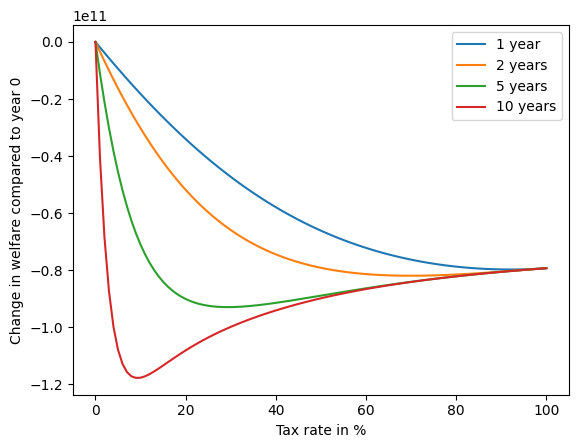
\includegraphics{Schedule1.png}
    \caption{Welfare effect of transfer schedule 1}
    \label{fig:sche1}
\end{figure}
Figure \ref{fig:sche1} shows the effect of the measure on the total welfare depending on the tax, expressed as a percentage of the income. After one year, the welfare effect is a monotonously decreasing function, the function for the effect on welfare after 10 years has a minimum welfare at about eight\%. For each of the functions, there is a plateau where the loss in welfare stays at a constant level of about -0.8 trillion pounds. Overall, however, every taxation, when redistributed only according to the risk in each region reduces the total welfare. 
\\
A possible reason for that result is that the regions in the UK with the highest risk are also the ones that are least productive, every transfer of money and in the consequence of citizens to those regions decreases the total productivity of the nation.
\subsubsection{Limitations and Consequences}
One can argue that the assumption of constant productivity per region is a weakness of the model because individuals might maintain their productivity when moving. Agent bases models can be more accurate in capturing dynamic with individual traits of individual citizens but those models far exceed the scope of this model.
\\
\subsection{Transfer Schedule 2: A more efficient transfer}
Addressing the major weakness of the first transfer schedule: Producing a decrease in welfare, this model aims at redistributing the collected taxes more efficiently.
The second transfer schedule transfers the money into the regions that have a high risk but also a high population density. The rationale is that the transfer most likely going to be invested into preventive measures, those are most efficient if they protect many citizens.
Technically, a risk value and value for the population density is assigned to each region according to population and risk data. The values are multiplied and normalized. This normalized value for a region is the percentage of received transfers from the total transfers.
\\
With this schedule the welfare increase increases monotonously with higher tax rates, plateauing at about 1.6 trillion pounds. The calculation for 10 years after introduction of the measure shows that tax rates of below 10\% are sufficient to reach the maximum welfare increase.
\begin{figure}
    \centering
    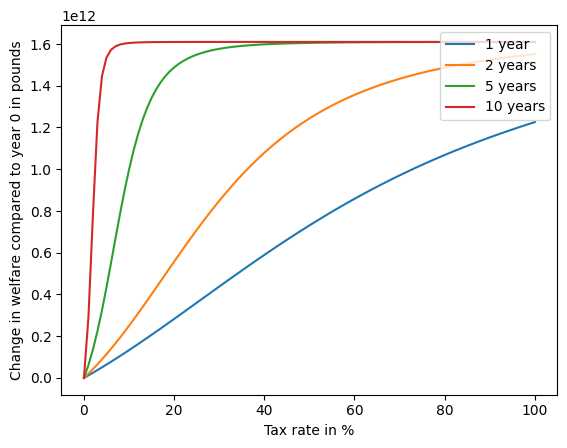
\includegraphics{Report/schedule2.png}
    \caption{Welfare effect of transfer schedule 2}
    \label{fig:sche2}
\end{figure}
\\
\subsection{Limitations and Additional models}
With the second transfer schedule yielding increases in welfare, one might be inclined to suggest policies similar to the transfer model. In reality, however, there are lots of feedback loops that have to be accounted for. Furthermore, in reality, there is moving stickiness, people do not easily move. Residential patterns are persistent over time regardless of whether their root cause is still effective. \cite{heblich_east-side_2021}
\\
In the data, there is a positive correlation between population density and productivity of a region. In our model we assumed to productivity per region to be constant, therefore, if everyone would move into the region with the highest productivity, the welfare would be maximized. In the real world, this has limitations.
\\
The first limitation we wanted to account for is the cost of housing in more densly populated areas. Plotting the cost of a house as a multiple of the average income in the region against the population density and applying a regression model yields a small increase in housing prices with rising population density. We constructed a model that subtracts a 30th of the purchasing price (calculated via the obtained regression function) of a house from the income per capita, as this is a usual repayment period. With this addition to the income, the first two transfer schedules were tested again. This approach yields a far less dynamic model in which the tax rate affects welfare less the the housing prices. In figure \ref{fig:housing} one can see that the housing price becomes the dominant factor, even contradicting further results: For some year the first schedule leads to an increase and the second schedule to a decrease in total welfare.
\begin{figure}
\centering
\begin{subfigure}{.45\textwidth}
    \centering
    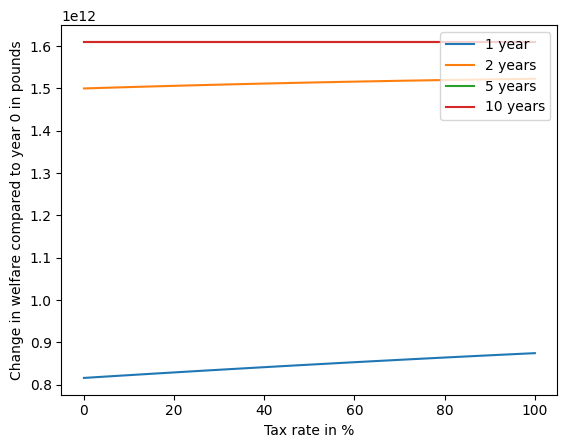
\includegraphics[width=\textwidth]{Report/schedule31.png}
    \caption{Welfare effect of transfer schedule 1 with housing prices}
\end{subfigure}
\begin{subfigure}{.45\textwidth}
    \centering
    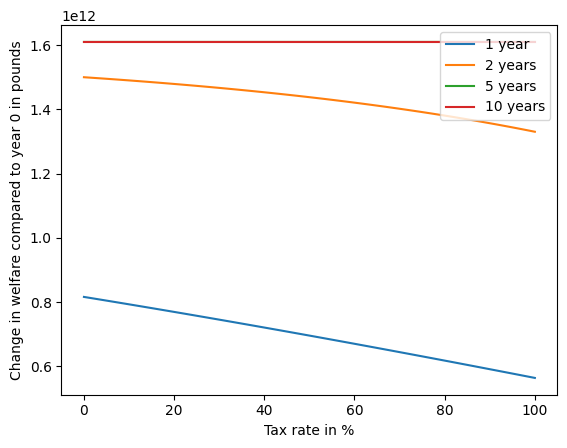
\includegraphics[width=\textwidth]{Report/schedule32.png}
    \caption{Welfare effect of transfer schedule 2 with housing prices}
\end{subfigure}
\caption{Effect of the housing prices on the transfer schedules}
\label{fig:housing}
\end{figure}
\subsubsection{Limitations}
By introducing housing prices to the model, we added an additional feedback loop. This loop changes the results notably and becoming the dominant factor for the total welfare. In a real-world scenario, there are a lot more feedback loops with a potential effect on the welfare: Transfers can be spent as investment, increasing attractivity of the regions; the productivity of individuals might stay constant independent of their place of residence; investments to mitigate risks like dams could decrease the risk in the regions; and many more. This enumeration illustrates that our models, in their current state, do not suffice to justify real world transfers of the magnitude mentioned in this paper.
\section{Conclusion}
Within the project, we developed three different transfer schedules for risk mitigation in the UK on NUTS 1 level. The three different analyzed transfers were a general tax and a distribution based on the risk per region, a distribution based on the risk and population density per region and an unequal tax redistribution based on risk. 
To analyze the transfer schedules' effect on overall welfare, we build a model to derive the attractivity of each region which is then transferred into welfare. The data is based on a monetary evaluation of the risks in each region. 
The analysis shows that population density needs to be taken into account in order to have a positive impact on welfare. This is derived from a comparison of the first two schedules of which the first lowers overall welfare by more than 5\% at a tax rate of 10\% while the second - considering population - improves overall welfare of up to 70\% at the same tax rate. Looking at the third transfer schedule which differentiates between different risk categories to derive individual tax rates, we see a different and almost negligible behavior in the welfare increase which reaches 0.0005\% welfare increase at a tax rate of 10\%. With a growing tax rate, the increase in welfare is linear and not exponential which makes the schedule less sensitive to changes in the tax rate but also less efficient in total welfare increase. These findings already show that an efficient money transfer within the UK can mitigate given risks and increase welfare. The sensitivity of welfare on the given transfer schedule is significant. An implementation of a transfer method must therefore be chosen carefully and tested in more sophisticated models. Furthermore, a multiplier effect can be detected from the different analyses. It shows that the effect of a schedule on welfare increases over time due to the dynamics of the model. The importance to find a working schedule and test it in a sophisticated model is therefore even underline since both, negative and positive consequences on welfare are amplified over time.
To conclude, the analysis shows that the transfer schedule must be chose carefully to achieve a positive impact on welfare and risk mitigation. To identify a reliable schedule to implement and optimize its behavior, more sophisticated models and simulations need to be executed.
\newpage
\section{Appendix}
List of tables and list of figures

\begin{figure}[H]
  \centering
  \includesvg[width=400pt]{wage-pop.svg}
  \caption{Wage - population density correlation}
  \label{dg:wage-pop}
\end{figure}

\begin{figure}[H]
  \centering
  \includesvg[width=400pt]{housing-pop.svg}
  \caption{Housing - population density correlation}
  \label{dg:housing-pop}
\end{figure}

\newpage
\printbibliography
\end{document}
